% 1998 年全国卷理科第 2 题：函数 y=a^{|x|}（a>1）的四个图象选项
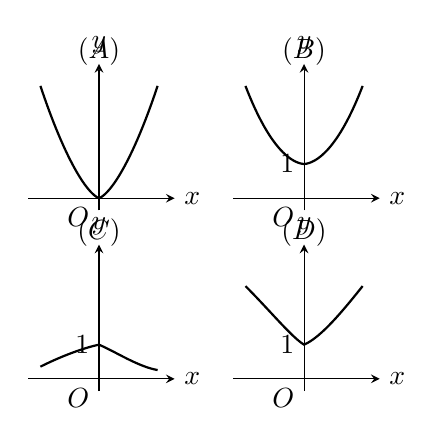
\begin{tikzpicture}[>=stealth, scale=0.62]
  \begin{scope}
    \node at (0,3.0) {$(A)$};
    \draw[->] (-1.45,0)--(1.55,0) node[right] {$x$};
    \draw[->] (0,-0.25)--(0,2.75) node[above] {$y$};
    \draw[thick] (-1.2,2.3) .. controls (-0.7,0.8) and (-0.25,0.1) .. (0,0)
      .. controls (0.25,0.1) and (0.7,0.8) .. (1.2,2.3);
    \node[below left] at (0,0) {$O$};
  \end{scope}

  \begin{scope}[xshift=4.2cm]
    \node at (0,3.0) {$(B)$};
    \draw[->] (-1.45,0)--(1.55,0) node[right] {$x$};
    \draw[->] (0,-0.25)--(0,2.75) node[above] {$y$};
    \draw[thick] (-1.2,2.3) .. controls (-0.7,1.0) and (-0.25,0.72) .. (0,0.7)
      .. controls (0.25,0.72) and (0.7,1.0) .. (1.2,2.3);
    \node[below left] at (0,0) {$O$};
    \node[left] at (0,0.7) {$1$};
  \end{scope}

  \begin{scope}[yshift=-3.7cm]
    \node at (0,3.0) {$(C)$};
    \draw[->] (-1.45,0)--(1.55,0) node[right] {$x$};
    \draw[->] (0,-0.25)--(0,2.75) node[above] {$y$};
    \draw[thick] (-1.2,0.25) .. controls (-0.7,0.5) and (-0.25,0.65) .. (0,0.7)
      .. controls (0.35,0.55) and (0.8,0.25) .. (1.2,0.18);
    \node[below left] at (0,0) {$O$};
    \node[left] at (0,0.7) {$1$};
  \end{scope}

  \begin{scope}[xshift=4.2cm,yshift=-3.7cm]
    \node at (0,3.0) {$(D)$};
    \draw[->] (-1.45,0)--(1.55,0) node[right] {$x$};
    \draw[->] (0,-0.25)--(0,2.75) node[above] {$y$};
    \draw[thick] (-1.2,1.9) .. controls (-0.7,1.4) and (-0.25,0.85) .. (0,0.7)
      .. controls (0.35,0.85) and (0.8,1.4) .. (1.2,1.9);
    \node[below left] at (0,0) {$O$};
    \node[left] at (0,0.7) {$1$};
  \end{scope}
\end{tikzpicture}
